\section{The Complex Plane}

\begin{definition}
    We define the \textbf{complex plane} to be the space of points $(x,y)$ of
    $\R^2$ for which  $z=x+iy$.
\end{definition}

\begin{lemma}\label{1.2.1}
    For every $z,w \in \C$  $|z+w| \leq |z|+|w|$.
\end{lemma}
\begin{proof}
    Observe that $-|z| \leq \re{z} \leq |z|$ for all $z \in \C$, so that
    $\re{z\bar{w}} \leq |z\bar{w}|=|z||w|$. So we get
    \begin{equation*}
        |z+w|^2=|z|^2+\re{z\bar{w}}+|\bar{w}| \leq
        |z|^2+|z||w|+|\bar{w}|=(|z|+|w|)^2
    \end{equation*}
    Taking square roots gives us the result.
\end{proof}
\begin{corollary}
    $|z+w|=|z|+|w|$ if  $z=tw$ for some  $t \geq 0$.
\end{corollary}
\begin{corollary}
    If $z_1, \dots, z_n \in \C$, then $|z_1+\dots+z_n| \leq
    |z_1|+\dots+|z_n|$.
\end{corollary}
\begin{proof}
    By induction on $n$.
\end{proof}
\begin{corollary}
    For all $z,w \in \C$,  $\big{|}|z|-|w|\big{|} \leq |z-w|$.
\end{corollary}
\begin{proof}
    We have that $|z| \leq |z-w|+|w|$, and $|w| \leq |z-w|+|z|$. So
    we get $|z|-|w| \leq |z-w|$ and $-|z-w| \leq |w|-|z|$, so that
    $\big{|}|z|-|w|\big{|} \leq |z-w|$.
\end{proof}

\begin{definition}
    We define the \textbf{polar form} of a complex number $z \in \C$ to be the
    polar coordinates  $(r,\th)$ where $r=|z|$ and  $\th$ is the angle between
    the line segment from  $0$ to  $z$ and the positive real axis. We call  $r$
    the \textbf{modulus} of $z$, and  $\th$ the  \textbf{argument} of $z$. We
    write $\th=\arg{z}$.
\end{definition}

\begin{lemma}\label{1.2.2}
    Let $z=r_1\cos{\th_1}+r_1i\sin{\th_1}$ and
    $w=r_2\cos{\th_2}+r_2i\sin{\th_2}$. Then
    \begin{equation*}
        zw=r_1r_2\cos{(\th_1+\th_2)}+r_1r_2i\sin{(\th_1+\th_2)}
    \end{equation*}
    so that  $\arg{zw}=\arg{z}+\arg{w}$.
\end{lemma}
\begin{proof}
    We multiply the expanded forms of $z$ and  $w$ together and use the
    trigonometric identities to get the result.
\end{proof}
\begin{corollary}
    If $z_k=r_k\cos{\th_k}+r_ki\sin{\th_k}$, then
    \begin{equation*}
        z_1 \dots z_n=(r_1 \dots r_n)\cos{(\th_1+\dots+\th_n)}+
        (r_1 \dots r_n)i\sin{(\th_1+\dots+\th_n)}
    \end{equation*}
\end{corollary}
\begin{proof}
    By induction on $n$.
\end{proof}

\begin{theorem}[DeMoivre's Theorem]\label{1.2.3}
    For all integers $n \geq 0$, if  $z=\cos{\th}+i\sin{\th}$, then
    \begin{equation*}
        z^n=\cos{n\th}+i\sin{n\th}
    \end{equation*}
\end{theorem}
\begin{proof}
    We use the corollory to lemma \ref{1.2.2} recursively on $z^n$.
\end{proof}

\begin{lemma}\label{1.2.4}
    FOr each nonzero $a \in \C$, and integer $n \geq 2$, the  polynomial $z^n-a$
    has has roots all  $z$ of the form
    \begin{equation*}
        z=|a|^{\frac{1}{n}}(\cos{\frac{\a+2k\pi}{n}}+
        i\sin{\frac{\a+2k\pi}{n}}) \text{ for all } 0 \leq k \leq n-1
    \end{equation*}
    where $a=|a|\cos{\a}+|a|i\sin{\a}$
\end{lemma}
\begin{proof}
    Let $a=|a|\cos{\a}+|a|i\sin{\a}$. Then we have $z^n-a=0$ has as solution
    \begin{equation*}
        z'=|a|^{\frac{1}{n}}(\cos{\frac{\a+2\pi}{n}}+i\sin{\frac{\a+2\pi}{n}})
    \end{equation*}
    The rest of the solutions are obtained by noting that $(z')^n-a=0$.
\end{proof}

\begin{definition}
    Let $a \in \C$ a nonzero complex number. We call the roots of the the
    polynomial $z^n-a \in \C[z]$ the \textbf{$n$-th roots} of $a$. We call the
    roots of  $z^n-1 \in \C[z]$ the \textbf{$n$-th roots of unity}.
\end{definition}

\begin{example}\label{example_1.2}
    The $n$-th roots of unity are all complex numbers of the form
    \begin{equation*}
        z=\cos{\frac{2k\pi}{n}}+i\sin{\frac{2k\pi}{n}} \text{ for all } 0 \leq k
        \leq n-1
    \end{equation*}
\end{example}

\begin{lemma}\label{1.2.5}
    Let $L \subseteq \C$ a straight line in  $\C$. Then  $L=\{z \in \C :
    \im{\frac{z-a}{b}}=0\}$, where $z=a+tb$ for some $t \in \R$.
\end{lemma}
\begin{proof}
    Let $a$ be any point in  $L$, and  $b$ the direction vector of  $L$. Then if
     $z \in L$  $z=a+tb$ for some  $t \in \R$. Since $b \neq 0$,
     $\im{\frac{z-a}{b}}=0$, since $t=\frac{z-a}{b}$, and $t \in \R$.
\end{proof}
\begin{corollary}
    Let $H_a=\{z \in \C : \im{\frac{z-a}{b}} > 0\}$ and $K_a=\{z \in \C :
    \im{\frac{z-a}{b}}<0\}$. Then $H_a=a+H_0$ and $K_a=a-K_0$.
\end{corollary}
\begin{proof}
    Suppose that $|b|=1$, and let  $a=0$, then  $H_0=\{z \in \C :
    \im{\frac{z}{b}} > 0\}$. Now, $b=\cos{\b}+i\sin{\b}$. If
    $z=r\cos{\th}+ri\sin{\th}$, then
    $\frac{z}{b}=r\cos{(\th-\b)}+ri\sin{(\th-\b)}$. So $z \in H_0$ if, and only
    if $\sin{(\th-\b)}>0$; that is $\b<\th<\pi+\b$, which makes  $H_0$ the upper
    half plane about $L$.
     \begin{figure}[h]
        \centering
        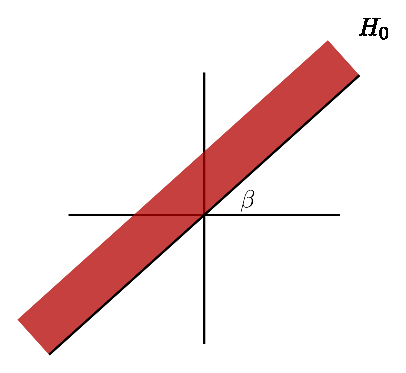
\includegraphics[scale=1]{Figures/chapter1/H_0.eps}
        \caption{}
        \label{}
    \end{figure}

    Putting $H_a=\{z \in \C : \im{\frac{z-a}{b}}>0\}$, we get $H_a=a+H_0$. By
    similar reasoning, we get $K_a=a-K_0$, where $K_a=\{z \in \C :
    \im{\frac{z-a}{b}}<0\}$.
\end{proof}
